\subsection{Two Ears Theorem}

Every simple polygon with more than 3 vertices has at least two non-overlapping ears (a ear is a vertex whose diagonal induced by its neighbors which lies strictly inside the polygon). Equivalently, every simple polygon can be triangulated. Example of a simple polygon with exactly two ears:

\begin{center}
    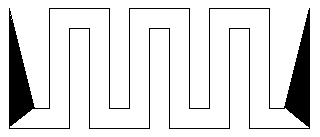
\includegraphics[width=0.6\linewidth]{img/two_ears.png}
    \end{center}
